\documentclass[11pt,a4paper]{article}
\usepackage[T1]{fontenc}
\usepackage[utf8]{inputenc}
\usepackage{lmodern}
\usepackage[margin=1in]{geometry}
\usepackage{amsmath}
\usepackage{graphicx}
\usepackage{booktabs}
\usepackage{microtype}
\usepackage[font=small,labelfont=bf]{caption}
\usepackage[numbers,sort&compress]{natbib}
\usepackage[hidelinks]{hyperref}
\setlength{\parskip}{0.35em}

\title{\textbf{PPO and GRPO against the Policy Optimiser of VerifiableRL:\\ A Pre-registered Comparison}}
\author{Sidi3355\thanks{Code, raw run records and the pre-registration:
\texttt{github.com/Sidi3355/grpo-trl}. See the disclosure at the end of the paper.}}
\date{November 2026}

\begin{document}
\maketitle

\begin{abstract}
\texttt{VerifiableRL}, the reinforcement-learning model of the Think-Reason-Learn library, learns which pieces
of information about a sample to reveal before predicting, and trains its policy by distilling Monte Carlo rollout
targets. We ask whether a whole-episode policy-gradient method, Proximal Policy Optimization (PPO) or Group
Relative Policy Optimization (GRPO), trains that policy better, holding the networks, rewards and deployment code
fixed and giving every method the same compute and the same tuning effort. The study was pre-registered. On six
datasets, two reward regimes and ten seeds, PPO scores 1.10 on a scale where 0 is a random policy and 1 the best
non-adaptive policy, against 0.60 for the shipped optimiser tuned and 0.49 as shipped. GRPO as published scores
0.60: dividing by each group's standard deviation gives slot-cost differences the weight of right-versus-wrong
calls, and its update has a mean cosine of 0.24 with the true policy gradient. Removing that division lifts GRPO
to 1.01, but the variant collapses late in training at four times the budget, where PPO reaches 1.42. The shipped
optimiser cannot learn when to stop, because its stopping target never sees costs. We recommend PPO and report
what the study cannot establish.
\end{abstract}

\section{Introduction}

Think-Reason-Learn (TRL) is an open-source library of scikit-learn classifiers built around language-model
reasoning \citep{trl2026}. One of its models, \texttt{VerifiableRL}, treats prediction as a sequence of
decisions: a sample's features come in named \emph{slots} (for a founder: education, jobs, prior exits), a policy
chooses which slot to reveal next or to stop, and a classifier predicts from what was revealed
\citep{ye2026learning}. Each prediction therefore comes with the list of slots it used.

This study asks one question: \emph{does a whole-episode policy-gradient method train the policy of
\texttt{VerifiableRL} better than the optimiser the library ships?} We test the two best-known candidates, PPO
\citep{schulman2017ppo} and GRPO \citep{shao2024deepseekmath}.

The study began from a narrower question, whether GRPO would improve on PPO in TRL, on the belief that TRL used
PPO. An audit of the code showed it does not; it uses rollout-based policy distillation. Both methods thus became
challengers to the shipped optimiser. The hypotheses were registered before any experiment, when GRPO was the
candidate of interest, and are reported as registered. The comparison of PPO with the shipped optimiser was not a
registered test and is reported as descriptive.

\paragraph{Findings.}
\begin{enumerate}\setlength{\itemsep}{0pt}
\item PPO beats the shipped optimiser at equal compute, at both budgets tried, in about half the wall-clock time.
\item The shipped optimiser cannot learn when to stop: in a cost-aware regime it reveals exactly its minimum
      number of slots on every dataset.
\item GRPO as published does not beat the shipped optimiser, for an identifiable reason: its per-group
      standard-deviation normalisation.
\item Without that normalisation GRPO matches PPO at a short budget and collapses over a long one.
\end{enumerate}

\section{Background}

\paragraph{The shipped optimiser.} We audited TRL at version 0.4.4 (commit \texttt{a712645}); the paper
describing the method could not be retrieved, so the description is of the code. For each state an episode
visits, every slot is revealed in turn and the current policy is rolled out ten times. The policy is fitted by
cross-entropy to a softmax of those rollout values, and its STOP output to a sigmoid of the reward for stopping
at once. The STOP target is therefore a function of the immediate call only; slot costs and step penalties shape
which slot is asked, not when to stop.

\paragraph{PPO} is an actor-critic method: a learned value function supplies per-step advantages
\citep{schulman2015gae} and the policy is improved on a clipped importance-weighted objective
\citep{schulman2017ppo}.

\paragraph{GRPO} removes the critic. For each prompt it samples a group of $G$ outputs and scores each against
its own group, $A_i = (r_i - \operatorname{mean}(r)) / \operatorname{std}(r)$, inside PPO's clipped objective
\citep{shao2024deepseekmath}. \citet{liu2025drgrpo} argue that the standard-deviation and length normalisations
bias the update, and remove both (``Dr.\ GRPO'').

\paragraph{GRPO outside language models.} \citet{deoliveira2025grpo} find that GRPO underperforms PPO on
classical control tasks except short-horizon CartPole, and suggest that grouping unrelated episodes is one cause,
since classical control has no prompt. \texttt{VerifiableRL} has the structure they lacked: every training
sample is a fixed starting context from which many episodes can be played, episodes are at most five steps long,
and the main reward arrives at the end.

\paragraph{Costly feature acquisition.} Learning which features to buy with reinforcement learning is an
established problem \citep{janisch2019costly}. This study does not compare against that literature's methods; it
varies only the optimiser inside one published model.

\section{Method}

\paragraph{What is fixed.} The policy and classifier networks, their initialisation, the action rule, the reward
and the deployment loop are imported from TRL and are identical for every arm. Only the policy optimiser varies.
Unit tests check, state by state, that the policy the new optimisers sample from has the same greedy action as
TRL's deployment rule, and that an episode's return equals what TRL's own rollout code pays for the same path.

\paragraph{Decision problem.} An episode starts with nothing revealed. The policy picks an unseen slot or STOP
(allowed after a minimum number of slots) until STOP, all slots are revealed, or a step limit. The return is the
reward of the classifier's call on what was revealed, minus the costs of the revealed slots and a penalty per
step.

\paragraph{Arms.} (i)~\emph{Shipped, defaults}: TRL's own trainer code with library defaults.
(ii)~\emph{Shipped, tuned}: the same code with searched settings. (iii)~\emph{PPO}: clipped objective, learned
critic, generalised advantage estimation. (iv)~\emph{GRPO, canonical}: the objective of
\citet{shao2024deepseekmath} with one group per training sample and no critic. (v)~\emph{GRPO, mean-centred}:
the same without division by the group's standard deviation; a single batch-wide scale is applied instead. Arm
(v) was a registered ablation that was promoted to a main arm, with its own hypotheses, after a pilot on one
development seed and before tuning.

\paragraph{Reward regimes.} \emph{R1} is TRL's defaults exactly: $+4$ for a true positive, $-16$ for a false
positive, $-0.1$ per step, at least three slots, no slot costs. \emph{R2} is a cost-aware regime built from
existing \texttt{VerifiableRL} arguments: the terminal reward is Youden's~$J$ (balanced accuracy, rescaled), each
slot has a cost, revealing everything costs half of what full information is worth, and STOP is allowed after one
slot.

\paragraph{Data.} Six datasets (Table~\ref{tab:data}), each with a fresh stratified split per seed into 2{,}000
training, 500 validation and 2{,}000 test samples (1{,}800/400/800 for founders). Text slots are embedded with
\texttt{all-MiniLM-L6-v2}.

\begin{table}[t]
\centering\small
\begin{tabular}{llrl}
\toprule
Dataset & Slots & Positive & Source \\
\midrule
Synthetic routing & 6 numeric & 29\% & generated; best strategy known \\
Founders & 6 text & 20\% & 3{,}000 generated founder profiles \\
Kickstarter & 3 text, 3 tabular & 32\% & public \\
Job postings (fraud) & 2 text, 3 tabular & 4\% & public \\
Credit default & 7 tabular (profile, six months) & 22\% & public \\
Census income & 5 tabular & 24\% & public \\
\bottomrule
\end{tabular}
\caption{Datasets. In synthetic routing a ``router'' slot names which of four candidate slots carries the label,
so the best strategy is to read the router, read the slot it names, and stop.}
\label{tab:data}
\end{table}

\paragraph{Budget.} Every run receives the compute the shipped optimiser spends on one default pass over the
training set, counted in multiply-accumulates by hooks on every network, PPO's critic included. We call this
\emph{one budget}. The endpoint is the policy at the end of the budget; no checkpoint is selected.

\paragraph{Tuning.} Each learner received 24 random configurations on four development conditions; the top three
were re-run on two further development seeds and one configuration per learner was frozen for all datasets and
regimes. Development seeds and confirmatory seeds are disjoint. The shipped optimiser received the same search
and, in addition, the right to set its own minimum number of slots in R2.

\paragraph{Classifier.} The reward depends on the classifier, so in the main experiment it is trained once per
dataset and seed by TRL's own pretraining and frozen for every arm. Section~\ref{sec:e2e} removes this
restriction.

\paragraph{Score and statistics.} Test return is normalised per condition so that 0 is a uniformly random policy
and 1 is the best fixed set of slots; values above 1 mean the policy gains by adapting. Runs are paired by seed.
Each registered test is the mean paired difference pooled over conditions with equal weight, with a bootstrap
confidence interval stratified by condition, a sign-flip permutation $p$-value, and Holm correction over eight
tests \citep{agarwal2021precipice}.

\paragraph{Pre-registration.} Hypotheses, metrics, analysis and a decision rule were committed to version control
before any experiment. Later changes are dated amendments, each made before the data it concerns; thirteen
departures from the first plan are logged with their reasons.

\section{Results}

\subsection{Main comparison}

Table~\ref{tab:main} and Figure~\ref{fig:main} give the main experiment: five arms, twelve conditions, ten seeds,
600 runs.

\begin{table}[t]
\centering\small
\begin{tabular}{lcccrr}
\toprule
Optimiser & Normalised return [95\% CI] & R1 & R2 & Below random & Seconds \\
\midrule
Shipped, defaults & 0.49 [0.39, 0.60] & 0.72 & 0.26 & 23\% & 38 \\
Shipped, tuned & 0.60 [0.48, 0.71] & 0.61 & 0.58 & 21\% & 41 \\
PPO & \textbf{1.10} [1.02, 1.17] & 1.17 & 1.03 & 4\% & 17 \\
GRPO, canonical & 0.60 [0.50, 0.70] & 0.92 & 0.27 & 23\% & 23 \\
GRPO, mean-centred & 1.01 [0.93, 1.09] & 1.07 & 0.96 & 8\% & 21 \\
\bottomrule
\end{tabular}
\caption{Main experiment at one budget, pooled over 12 conditions and 10 seeds. ``Below random'': share of runs
ending below the random policy. ``Seconds'': wall-clock per run at equal compute.}
\label{tab:main}
\end{table}

\begin{figure}[t]
\centering
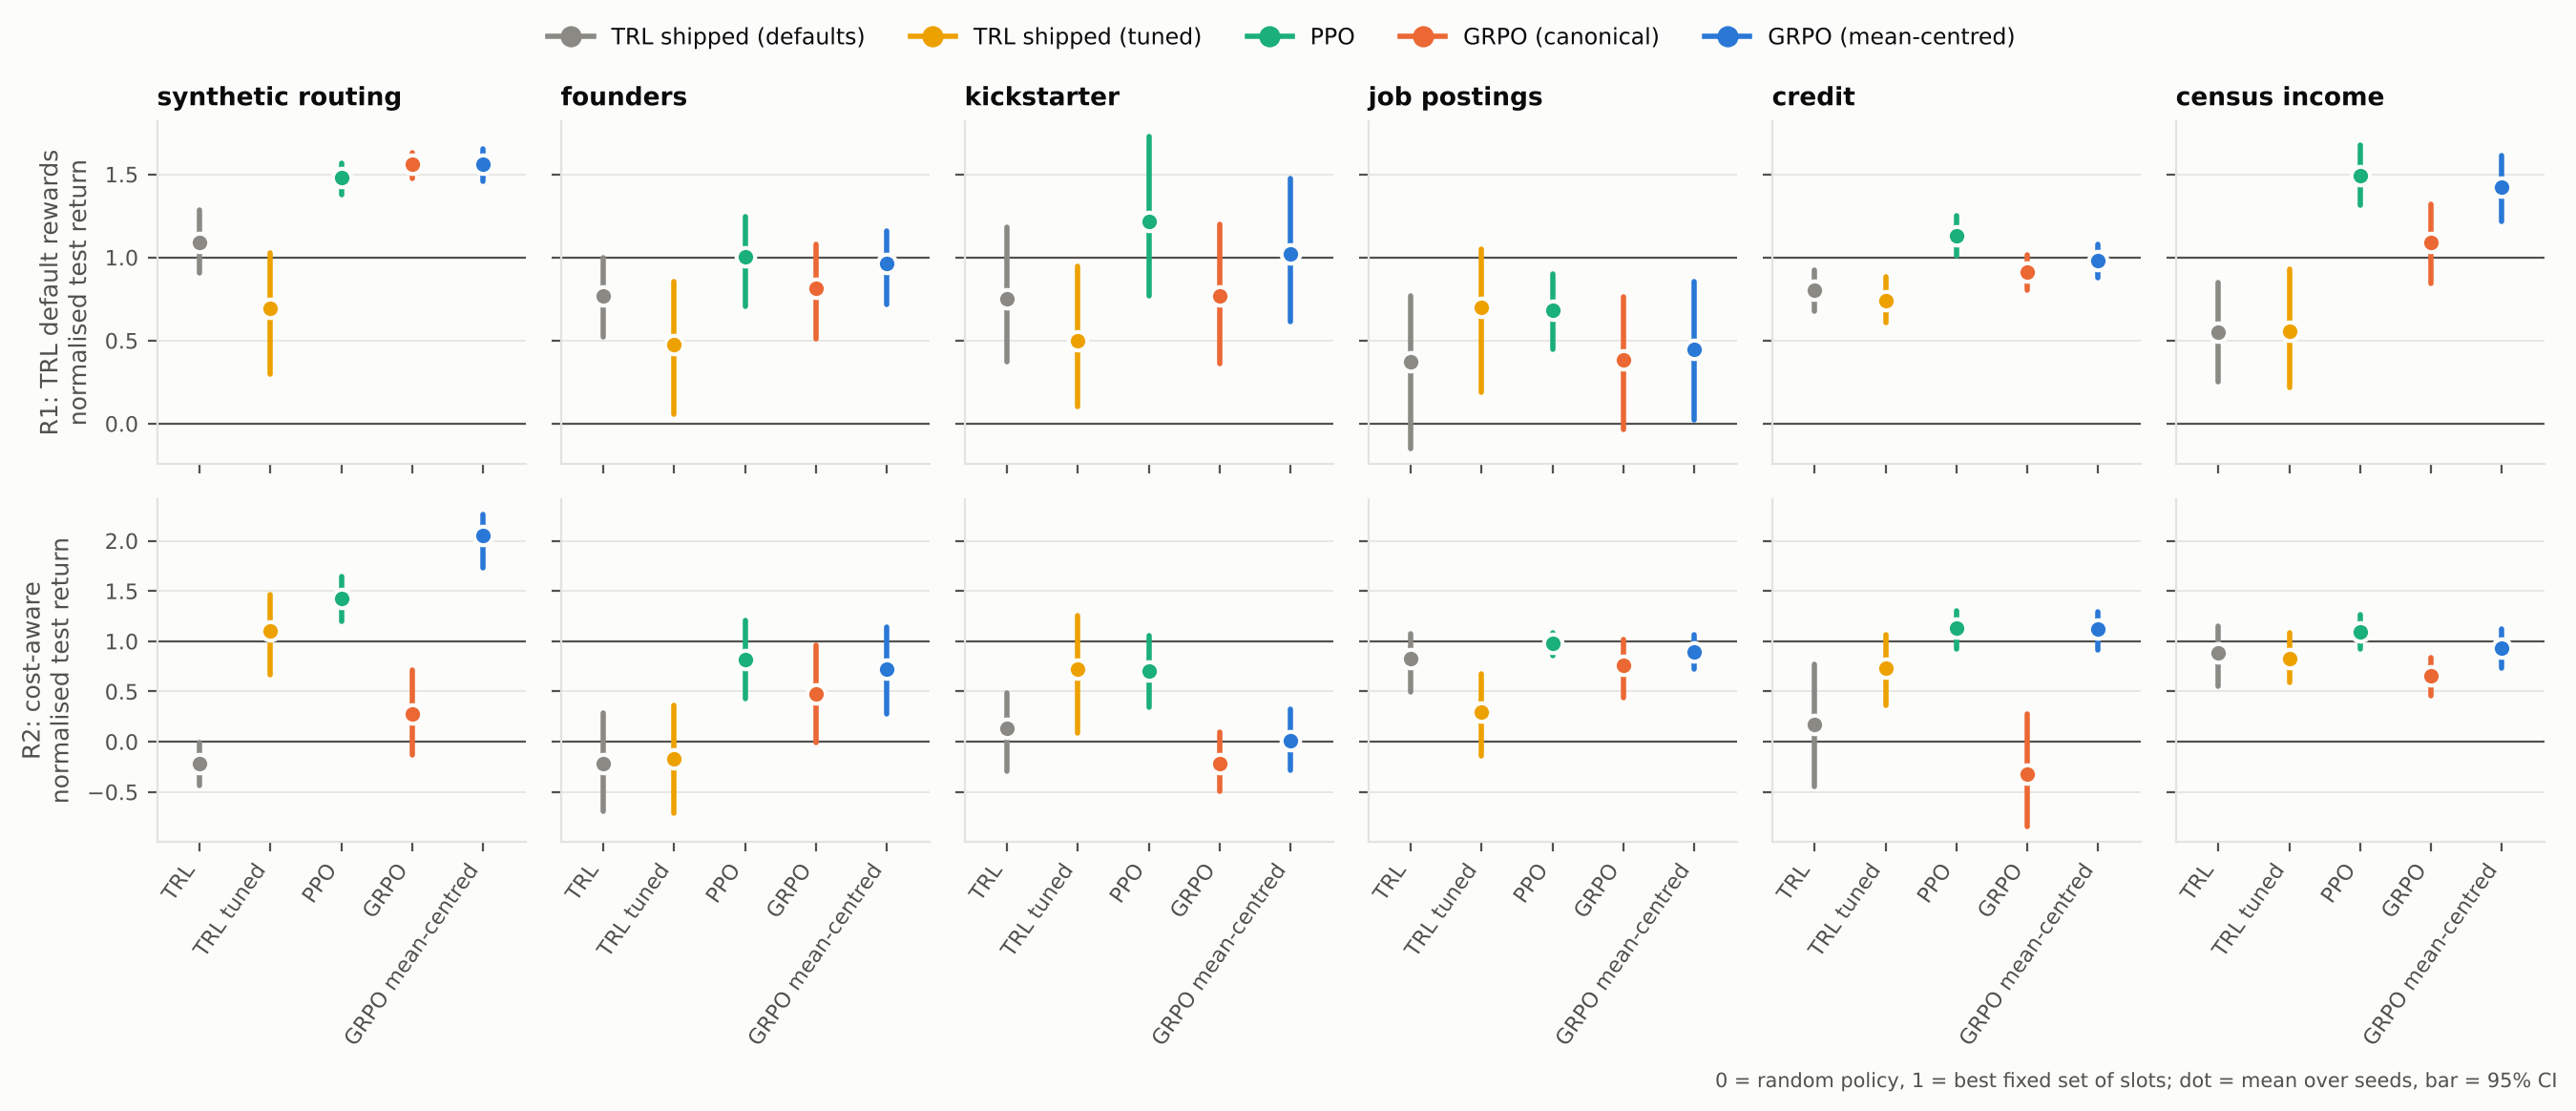
\includegraphics[width=\textwidth]{figures/fig1_main_results.png}
\caption{Normalised test return by dataset and regime (mean and 95\% CI over ten seeds). 0 is the random policy,
1 the best fixed set of slots.}
\label{fig:main}
\end{figure}

\textbf{PPO against the shipped optimiser} (descriptive, unadjusted): $+0.50$ $[+0.40, +0.60]$ over the tuned
configuration, with 9 of 12 conditions won and none lost; $+0.56$ in R1 and $+0.44$ in R2. Tuning helped the
shipped optimiser in R2 and hurt it in R1, so the fairest incumbent differs by regime; PPO leads the better one
by $0.45$ and $0.44$.

\textbf{On the problem with a known optimum}, synthetic routing in R2, mean-centred GRPO reveals 2.16 slots per
sample and scores 2.05; PPO reveals 3.99 and scores 1.42; the tuned shipped optimiser scores 1.10 and canonical
GRPO 0.28.

\subsection{Registered tests}

\begin{table}[t]
\centering\small
\begin{tabular}{llccl}
\toprule
& Claim & Difference [95\% CI] & Holm $p$ & Verdict \\
\midrule
H1 & GRPO beats PPO & $-0.50$ [$-0.59$, $-0.41$] & 0.0008 & reversed \\
H2a & GRPO beats shipped, R2 & $-0.31$ [$-0.53$, $-0.09$] & 0.063 & not supported \\
H2b & GRPO non-inferior to shipped, R1 & $+0.31$ [$+0.20$, $+0.42$] & 0.0008 & supported \\
H3 & Per-sample groups beat batch groups & $-0.85$ [$-1.06$, $-0.61$] & 0.0008 & reversed \\
H4 & Mean-centred and canonical GRPO differ & $+0.94$ [$+0.73$, $+1.14$] & 0.0008 & supported \\
H1$'$ & Mean-centred GRPO beats PPO & $-0.09$ [$-0.15$, $-0.02$] & 0.063 & not supported \\
H2a$'$ & Mean-centred GRPO beats shipped, R2 & $+0.37$ [$+0.18$, $+0.57$] & 0.012 & supported \\
H2b$'$ & Mean-centred GRPO non-inferior, R1 & $+0.46$ [$+0.35$, $+0.56$] & 0.0008 & supported \\
\bottomrule
\end{tabular}
\caption{Registered tests: pooled paired difference in normalised test return, first arm minus second.
``Shipped'' is the tuned configuration. Non-inferiority margin 0.10. H1--H4 were registered before any experiment; the primed tests were added after a
pilot on one development seed and before tuning.}
\label{tab:tests}
\end{table}

Table~\ref{tab:tests} lists the eight registered tests. Two of the four original predictions came out the
opposite way. Mean-centred GRPO passes both of its tests against the shipped optimiser; neither GRPO variant
beats PPO.

\subsection{Stopping}

In R2 the shipped optimiser with default settings reveals between 1.00 and 1.01 slots on every dataset: it stops
at its minimum. Tuned, where the search gave it a floor of two, it reveals between 2.04 and 2.33. PPO varies from
1.21 to 3.99 slots by dataset and mean-centred GRPO from 1.13 to 2.16. The shipped optimiser learns which slot
to ask first; it does not learn when to stop.

\subsection{Why canonical GRPO fails here}

\paragraph{Mechanism.} With no training, we played 16 episodes per training sample at the initial policy and
compared each advantage rule's update direction with the true policy gradient (Table~\ref{tab:cos}). In 39\% of
groups every episode ends in the same call, so their returns differ only by slot costs or step penalties.
Dividing by that small spread turns a step penalty of 0.1 into an advantage as large as the gap between a true
and a false positive. In R1 the true mean advantage of the shortest and longest episodes in a group is $-0.01$
and $+0.01$; canonical GRPO assigns them $+0.36$ and $-1.32$. The policy learns to stop as early as it is
allowed, which is harmless in R1 (three slots is about right) and costly in R2.

\begin{table}[t]
\centering\small
\begin{tabular}{lcc}
\toprule
Advantage rule & Mean cosine & Range \\
\midrule
Per-sample mean and std (GRPO, canonical) & 0.24 & $-0.86$ to 0.69 \\
Per-sample mean (GRPO, mean-centred) & 0.99 & 0.98 to 1.00 \\
Batch mean and std & 0.98 & 0.96 to 1.00 \\
No baseline & 0.75 & 0.33 to 0.99 \\
\bottomrule
\end{tabular}
\caption{Cosine between each advantage rule's update and the true policy gradient at the initial policy: mean
and range over 12 conditions (3 seeds each).}
\label{tab:cos}
\end{table}

\paragraph{Ablation.} Holding the data collection, the clipped objective and canonical GRPO's settings fixed and
changing only the baseline (Figure~\ref{fig:ladder}; four conditions, ten seeds), the two arms that divide by the
group's standard deviation score 0.31 and 0.25 and every other arm scores between 1.03 and 1.25. A per-sample
mean (1.25) is ahead of a critic that is given the label (1.19), an ordinary critic (1.13) and a batch baseline
(1.16), but none of those gaps is established. Length normalisation makes no difference. Group size does not
matter for the mean-centred variant: sizes from 2 to 32 score between 1.11 and 1.25.

\begin{figure}[t]
\centering
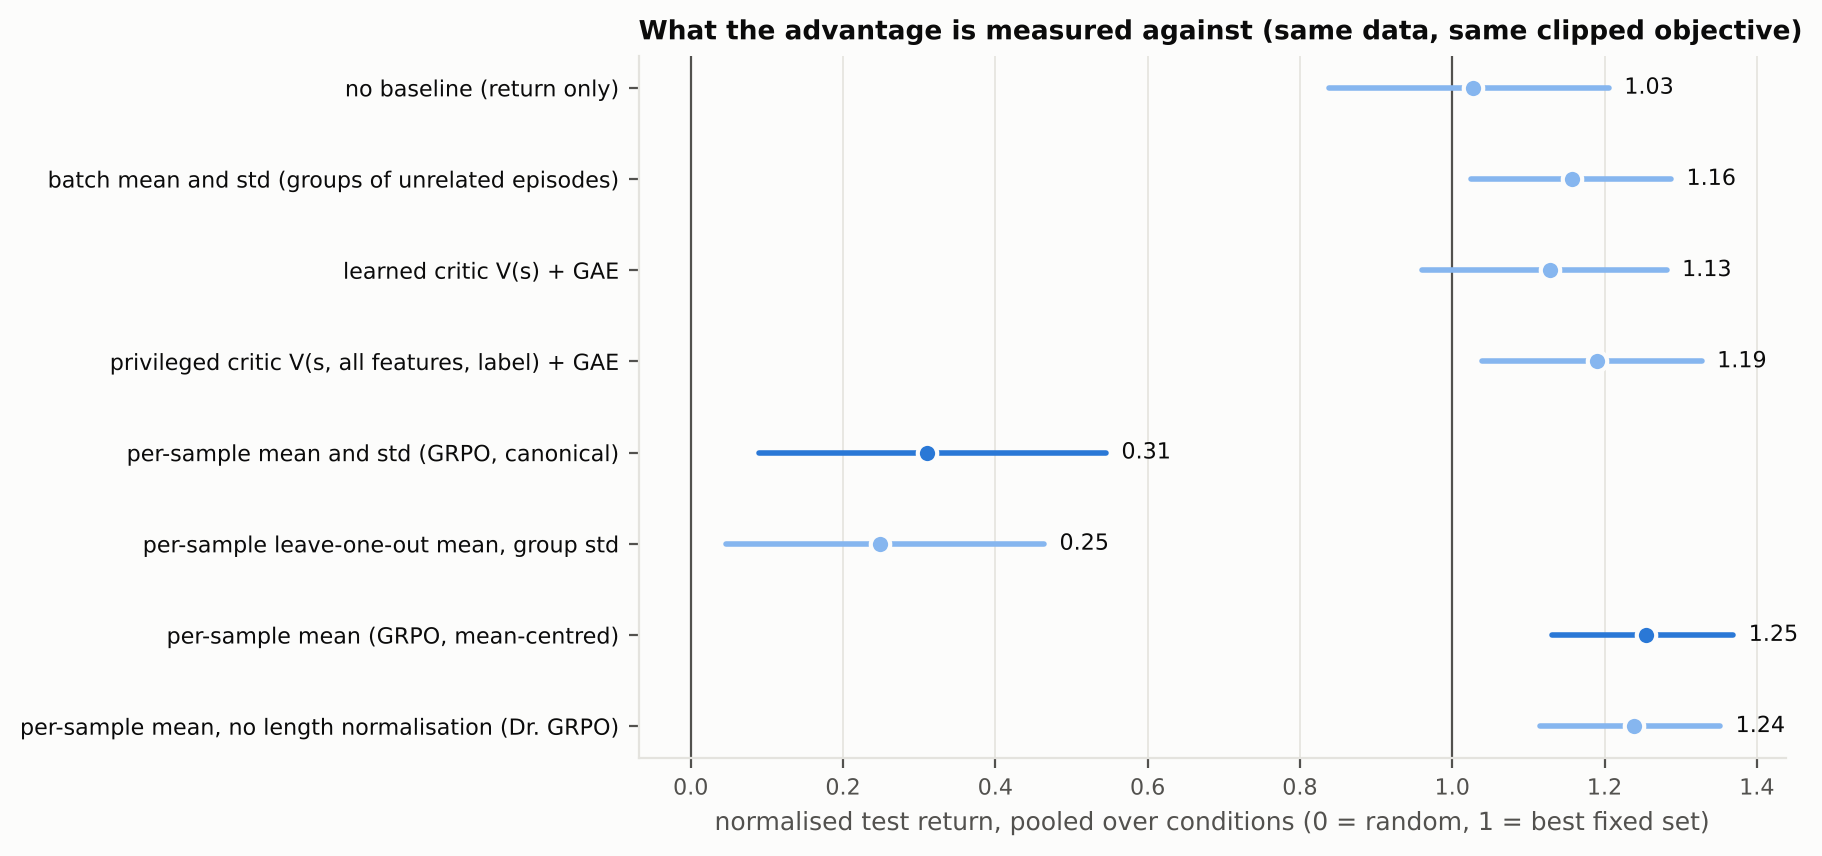
\includegraphics[width=0.86\textwidth]{figures/fig4_baseline_ladder.png}
\caption{What the advantage is measured against, with everything else fixed (pooled normalised test return,
95\% CI).}
\label{fig:ladder}
\end{figure}

\subsection{Four times the budget}

\begin{table}[t]
\centering\small
\begin{tabular}{lccc}
\toprule
Optimiser & One budget & Four budgets & Runs ending $>0.3$ below their best \\
\midrule
Shipped, defaults & 0.36 [0.12, 0.58] & 0.37 [0.12, 0.61] & 4 of 12 \\
Shipped, tuned & 0.55 [0.25, 0.84] & 0.87 [0.58, 1.18] & 3 of 12 \\
PPO & 1.20 [0.92, 1.45] & \textbf{1.42} [1.24, 1.60] & 2 of 12 \\
GRPO, canonical & 0.68 [0.42, 0.91] & 0.75 [0.46, 1.03] & 2 of 12 \\
GRPO, mean-centred & 1.35 [1.01, 1.64] & 0.95 [0.63, 1.23] & 8 of 12 \\
\bottomrule
\end{tabular}
\caption{The same four conditions and three seeds at one and at four budgets.}
\label{tab:budget}
\end{table}

Table~\ref{tab:budget} gives each arm four times the budget. The shipped optimiser with default settings does not
improve, so it was not merely under-trained. PPO keeps improving and leads the tuned shipped optimiser by $0.55$
$[0.31, 0.75]$. Mean-centred GRPO reaches PPO's level part-way through and then drops sharply in 8 of 12 runs,
finishing $0.47$ $[0.22, 0.73]$ behind PPO. The gap between training and test return does not widen, so this is
instability and not over-fitting.

We registered one diagnosis before reading the remaining seeds: the batch-wide scale that the mean-centred
advantages are divided by shrinks as the policy converges, so the step size never does. Dividing by the batch
standard deviation of the returns instead made no difference at one budget (1.01 against 0.99) and helped a
little at four (1.12 against 0.95), but 6 of 12 runs still collapsed. The diagnosis is at most part of the cause.
This follow-up is post hoc and small.

\subsection{End to end}
\label{sec:e2e}

\begin{table}[t]
\centering\small
\begin{tabular}{lrrcrr}
\toprule
& \multicolumn{2}{c}{Test return} & & \multicolumn{2}{c}{Seconds per fit} \\
Condition & Shipped & Critic-free & Difference [95\% CI] & Shipped & Critic-free \\
\midrule
Founders, R1 & $-1.67$ & $-1.07$ & $+0.60$ [$+0.28$, $+0.83$] & 297 & 131 \\
Founders, R2 & 0.156 & 0.240 & $+0.08$ [$+0.02$, $+0.14$] & 180 & 100 \\
Credit, R1 & $-1.00$ & $-1.07$ & $-0.07$ [$-0.23$, $+0.12$] & 101 & 32 \\
Credit, R2 & 0.304 & 0.338 & $+0.03$ [$-0.02$, $+0.11$] & 61 & 20 \\
\bottomrule
\end{tabular}
\caption{Through the library's public \texttt{fit}, with the classifier co-trained (five seeds). The shipped
optimiser has three passes over the training set, the critic-free optimiser one; differences are paired by seed.}
\label{tab:e2e}
\end{table}

TRL co-trains the classifier on the states the policy reaches. We implemented mean-centred GRPO inside the
library and ran both optimisers through the public interface (Table~\ref{tab:e2e}), giving the shipped optimiser
three passes and the critic-free optimiser one. The critic-free optimiser wins 12 of 20 paired seeds on test
return and 16 of 20 on $F_{0.5}$, in a third to a half of the time. The margin is smaller than with a frozen
classifier. PPO was not run this way.

\section{Discussion}

\paragraph{Against the shipped optimiser.} PPO's lead is large at both budgets and in both regimes. Two
properties of the shipped optimiser explain most of it. Its stopping target is a function of the immediate call
only, so costs cannot reach the stopping decision. And it spends its budget labelling each visited state with
sixty rollouts, where a whole-episode method learns from every decision of every episode it plays.

\paragraph{PPO against GRPO.} GRPO as published is not suited to this problem, because every episode carries
small, real cost differences that per-group standardisation inflates; in language-model training, where rewards
are typically right or wrong, a group that agrees has zero spread and the issue does not arise. With the
standardisation removed, a critic-free method with per-sample groups comes within 0.09 of PPO at one budget,
which supports the suggestion of \citet{deoliveira2025grpo} that grouping matters. It does not overtake PPO, and
it is not stable over a long run.

\paragraph{The default reward.} Under R1 a positive call pays on average only when it is right about 80\% of the
time. On every real dataset here the classifier is right far less often, so mean returns are negative for every
arm and the return-maximising policy leads the classifier to call positive as rarely as possible. A better
optimiser finds that policy more reliably: on founders in R1, PPO has the highest return and the lowest
$F_{0.5}$ (0.15 against 0.24). This is a property of the reward, not of any optimiser.

\paragraph{Recommendation.} Offer a whole-episode policy-gradient optimiser in \texttt{VerifiableRL}, and make
it PPO. The registered decision rule, taken to the letter, selects mean-centred GRPO, which passed both of its
tests at one budget; the four-budget experiment shows that variant is not yet safe to train for long, so we
report the rule's answer and do not follow it. Canonical GRPO should not be offered.

\section{Limitations}

\begin{itemize}\setlength{\itemsep}{0pt}
\item \textbf{Power.} Ten seeds resolve pooled differences of roughly 0.17 or more; the registered target would
      have needed over 100. The ranking of PPO and mean-centred GRPO at one budget is not settled.
\item \textbf{Small follow-ups.} The four-budget, end-to-end and post hoc experiments use three to five seeds on
      four conditions. The cause of the late collapse is not established and no remedy was validated.
\item \textbf{Frozen classifier.} The main experiment freezes it; only the critic-free optimiser was run end to
      end.
\item \textbf{Data and scale.} The founder profiles are generated, the benchmark the method was built for
      (VCBench) was not available, and all experiments use 2{,}000 training samples and small networks.
\item \textbf{Scope.} The original paper could not be read; the incumbent is the library code. PPO against the
      shipped optimiser was not a registered test. No method from the costly-feature-acquisition literature was
      compared. PPO and GRPO are single implementations written for this study.
\end{itemize}

\section*{Disclosure}

The experiments, analysis code and the draft of this report were produced with substantial assistance from an AI
coding assistant (Claude Code) working under the author's direction. The author is responsible for the content.
All code, the pre-registration with its amendments, and one record per run are in the repository.

\bibliographystyle{plainnat}
\bibliography{references}

\end{document}
